% !TeX root = ../main.tex

\section{Approach}
\label{sec:approach}

This section presents the detailed design of \tool{}, our hierarchical framework for project-level Java to C++ code translation. We first provide an overview of the framework architecture, then describe each component in detail.

\begin{figure*}[h]
\centering
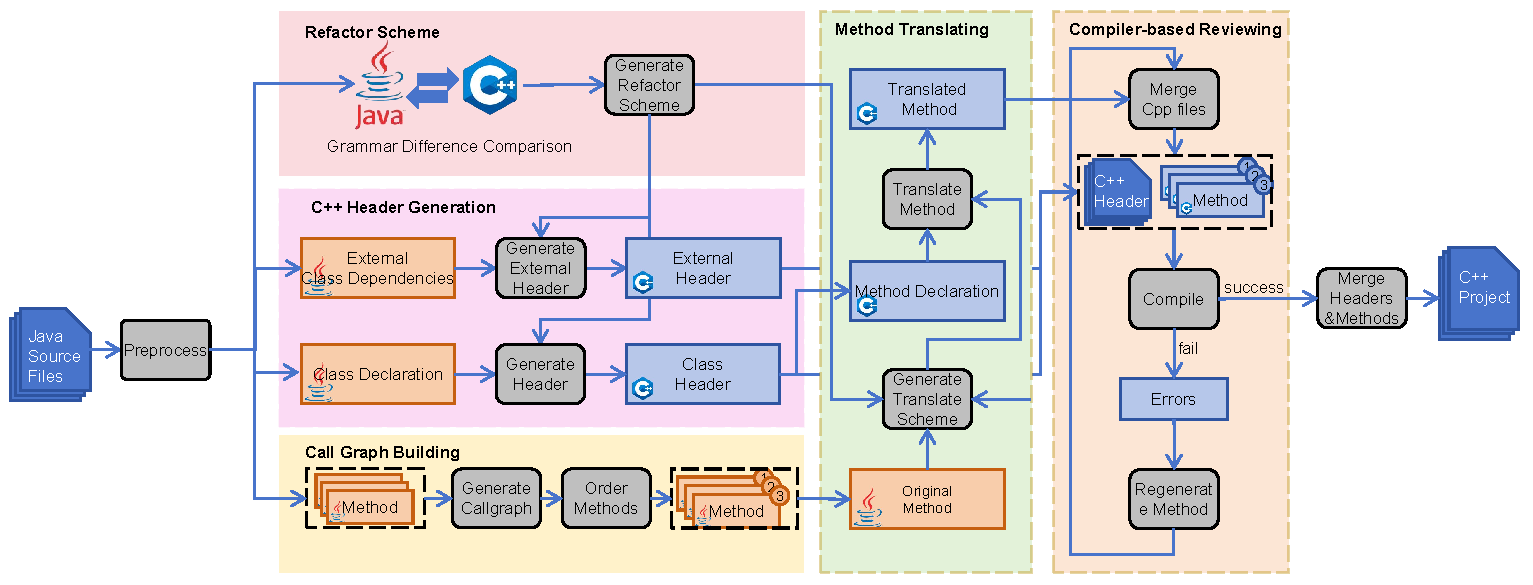
\includegraphics[width=\textwidth]{figures/approach/architecture-overall.pdf}
\caption{Overall architecture of \tool{} showing the three-phase translation process.}
\label{fig:architecture-overview}
\end{figure*}

\subsection{Framework Overview}

Figure~\ref{fig:architecture-overview} illustrates the overall architecture of \tool{}. The framework adopts a \textbf{macro-to-micro translation strategy} that separates high-level structural design from low-level implementation details. This hierarchical decomposition addresses two key challenges in project-level code translation: (1) managing complexity at scale, and (2) mitigating error propagation through context-aware translation ordering.

The translation process consists of three main phases:

\begin{enumerate}
\item \textbf{Static Analysis Phase}: A custom Java parser tool extracts the project structure, including class hierarchies, method signatures, and call graph dependencies. This phase decomposes the codebase into a hierarchical graph representation comprising \emph{Header nodes} (classes, interfaces, enums) and \emph{Method nodes} (individual method implementations). The graph captures both structural relationships (inheritance, type dependencies) and behavioral relationships (method call dependencies), which guide subsequent translation ordering.

\item \textbf{Hierarchical Translation Phase}: The framework performs translation in two interdependent layers:
\begin{itemize}
\item \textit{Header-level translation}: For each Java class, interface, and enum, the LLM generates a translation scheme that maps Java language constructs to appropriate C++ patterns (e.g., interfaces to abstract base classes with virtual functions, checked exceptions to error code handling). This layer establishes the structural foundation and type mapping conventions for the entire project.
\item \textit{Method-level translation}: Methods are translated following a bottom-up ordering derived from the call graph. Callee methods are translated before their callers, enabling that already-translated code serves as reference for translating dependent methods. This dependency-aware approach significantly reduces translation inconsistencies and API mismatches.
\end{itemize}

\item \textbf{Validation and Repair Phase}: An autonomous compilation agent iteratively compiles the translated C++ code, analyzes compilation errors, and applies fixes using LLM-generated suggestions. The agent operates through a tool-use interface, invoking compilation and file modification primitives to iteratively resolve errors until compilation succeeds or maximum attempts are reached.
\end{enumerate}

\subsection{Static Analysis and Graph Construction}

The first phase of \tool{} involves parsing the Java source code and extracting structural information necessary for guiding the translation process. This phase constructs a project-level dependency graph that serves as the foundation for all subsequent translation decisions.

\subsubsection{Project Graph Model}

The static analysis phase constructs a bipartite graph representation consisting of two types of nodes:

\begin{itemize}
\item \textbf{Header Nodes}: Represent type declarations (classes, interfaces, enums). Each Header node captures:
\begin{itemize}
\item The complete type declaration and field members
\item Inheritance relationships (parent class, implemented interfaces)
\item Import dependencies (external types required by this compilation unit)
\item A reference to all contained Method nodes
\end{itemize}

\item \textbf{Method Nodes}: Represent individual method implementations. Each Method node captures:
\begin{itemize}
\item The method signature (return type, parameter types, modifiers)
\item The complete method body implementation
\item Call dependencies (\texttt{children}: methods called by this method; \texttt{parents}: methods that call this method)
\item External call references (calls to methods outside the project boundary)
\end{itemize}
\end{itemize}

This bipartite structure enables separate handling of structural translation (Headers) and behavioral translation (Methods), while maintaining explicit relationships between them.

\subsubsection{Call Graph Extraction}

To establish the correct translation order for methods, the framework extracts the complete call graph from the Java source code. We integrate \texttt{java-callgraph2}, a static analysis tool that identifies method call relationships through points-to analysis.

The call graph construction process involves:
\begin{enumerate}
\item Parsing method call traces from \texttt{java-callgraph2} output
\item Matching caller and callee signatures to Method nodes in the project graph
\item Establishing bidirectional edges between caller-callee pairs
\item Identifying external dependencies (calls to library methods outside the project)
\end{enumerate}

The resulting call graph enables topological sorting of methods into translation layers, where all dependencies of a method in layer $n$ are guaranteed to be in layers $1$ through $n-1$.

\subsection{Hierarchical Translation Pipeline}

The translation pipeline operates on the project graph in two distinct phases: Header-level translation establishes the structural foundation and type conventions, followed by Method-level translation that leverages dependency ordering for context propagation. Each phase employs a dual-pass strategy consisting of scheme generation followed by code generation.

\subsubsection{Header-Level Translation}

Header-level translation addresses the structural differences between Java and C++, establishing consistent conventions for the entire project before translating individual method implementations.

\paragraph{Scheme Generation.} For each Header node, the LLM generates a \textbf{translation scheme}, a structured document that specifies:
\begin{itemize}
\item \textbf{Type mapping strategy}: How Java types map to C++ types (e.g., \texttt{ArrayList<T>} $\rightarrow$ \texttt{std::vector<T>})
\item \textbf{External dependency handling}: Identification of external dependencies that cannot be directly translated (e.g., third-party libraries, Java framework types), with strategies for mocking, replacing, or omitting them
\item \textbf{Memory management strategy}: How to replace Java's garbage collection with appropriate C++ memory management (e.g., using stack allocation where possible, smart pointers for heap-allocated objects, RAII patterns for resource management)
\item \textbf{Inheritance mapping}: How to map Java interfaces and abstract classes to C++ (e.g., interfaces $\rightarrow$ abstract base classes with pure virtual methods, default methods $\rightarrow$ virtual methods with implementations)
\item \textbf{Generics conversion}: How to convert Java generics to C++ templates (including handling of bounded type parameters, wildcards, and type erasure implications)
\end{itemize}

The scheme serves as a contract between high-level design and detailed implementation, ensuring consistency across all methods within the class.

\paragraph{Header Translation.} Using the generated scheme, the LLM translates each Header node to a C++ header file. The translation handles:
\begin{itemize}
\item Converting class declarations to C++ class syntax
\item Translating field declarations with appropriate C++ types and initialization requirements
\item Generating method declarations with translated signatures
\item Adding necessary \texttt{\#include} directives for both standard library and project dependencies
\item Handling namespace declarations and forward declarations where appropriate
\end{itemize}

Importantly, in our framework, the translated C++ project structure may differ from the original Java structure while preserving core functionality. The dual-pass approach grants the LLM considerable flexibility during Header translation, particularly in scheme generation where structural refactoring decisions are made. For example:
\begin{itemize}
\item Java utility classes containing only static methods may be translated to C++ namespaces with free functions, eliminating the need for class instantiation
\item Methods may be added, removed, or reorganized to better align with C++ idioms (e.g., separating declaration and definition, adding helper functions)
\item Multiple Java classes in one file may be split into separate C++ header files, or vice versa, depending on compilation dependencies
\item Interfaces may be merged or eliminated in favor of template-based designs where appropriate
\end{itemize}

This structural flexibility is particularly valuable when translating between languages with significant paradigmatic differences (e.g., object-oriented Java to multi-paradigm C++ with template metaprogramming), as it enables the translated code to follow idiomatic C++ patterns rather than mechanically mimicking Java's structure.

\begin{figure*}
  \centering
  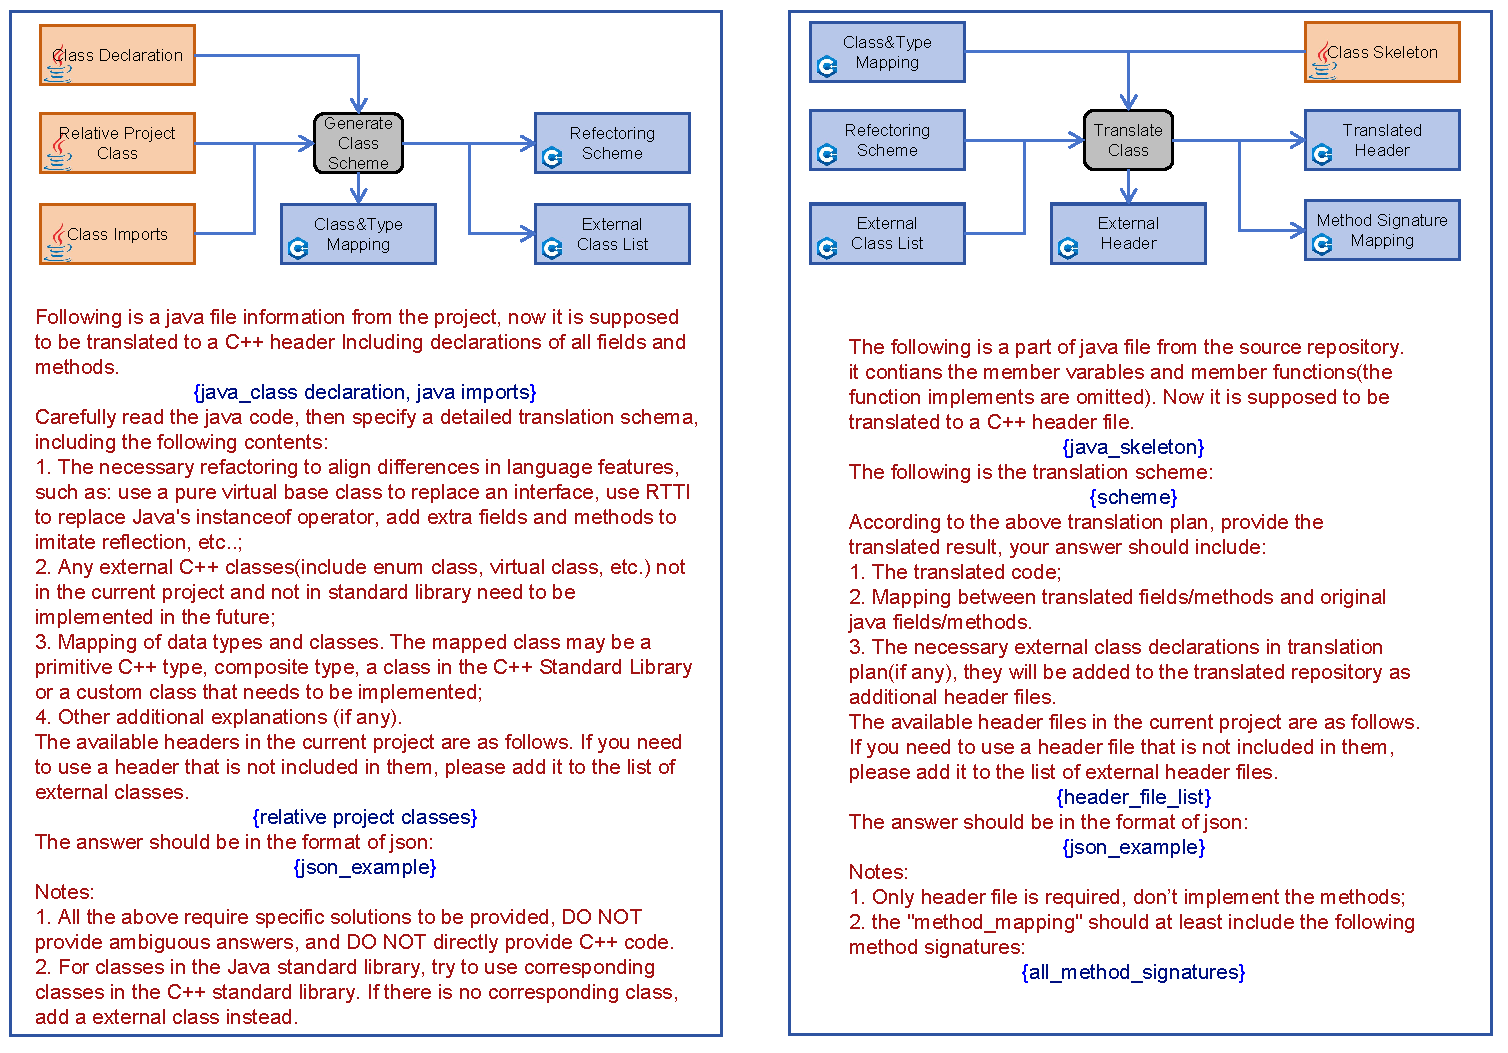
\includegraphics[width=\textwidth]{figures/approach/class_translation_prompt.pdf}
  \caption{Header-level translation scheme and data flow. The LLM analyzes the Java class structure, generates a translation scheme specifying type mappings and structural changes, then produces the corresponding C++ header file.}
  \label{fig:class-translation}
\end{figure*}

\subsubsection{Method-Level Translation}

Method-level translation focuses on translating implementation logic while maintaining behavioral equivalence. The key innovation is the bottom-up translation order, which enables effective context propagation.

\paragraph{Dependency-Aware Translation Ordering.} Methods are grouped into layers using topological sort on the call graph:
\begin{itemize}
\item \textbf{Layer 1}: Leaf methods with no internal calls (pure computations, external library calls only)
\item \textbf{Layer $n$}: Methods whose callees all reside in layers $1$ through $n-1$
\end{itemize}

Methods within the same layer have no mutual dependencies and can be translated in parallel, providing opportunities for concurrent processing.

\paragraph{Scheme Generation.} For each Method node, the LLM generates a detailed translation scheme that includes:
\begin{itemize}
\item \textbf{Functionality summary}: A concise description of what the method accomplishes
\item \textbf{Implementation strategy}: How to achieve the same behavior in C++ (e.g., replacing Java streams with C++ algorithms, converting iterator-based loops with range-based for loops)
\item \textbf{Context requirements}: Which already-translated methods to reference as examples
\item \textbf{Exception handling}: How to convert Java checked exceptions to C++ error handling (e.g., return values, error codes, or C++ exceptions)
\end{itemize}

Because all callees are translated before their callers, the scheme can explicitly reference specific translation patterns from already-translated methods, promoting consistency across the codebase.

\paragraph{Method Translation.} Methods are translated layer by layer. For each method, the LLM receives:
\begin{itemize}
\item The original Java method code
\item The method's translation scheme
\item \textbf{Translated code of all callees}: This provides concrete examples of how similar constructs were translated, enabling \emph{pattern-based consistency}
\item The translated Header for context on available types and APIs
\end{itemize}

This context-rich prompting significantly reduces hallucination by providing the LLM with concrete examples of how similar language constructs were translated elsewhere in the project.

\begin{figure*}
  \centering
  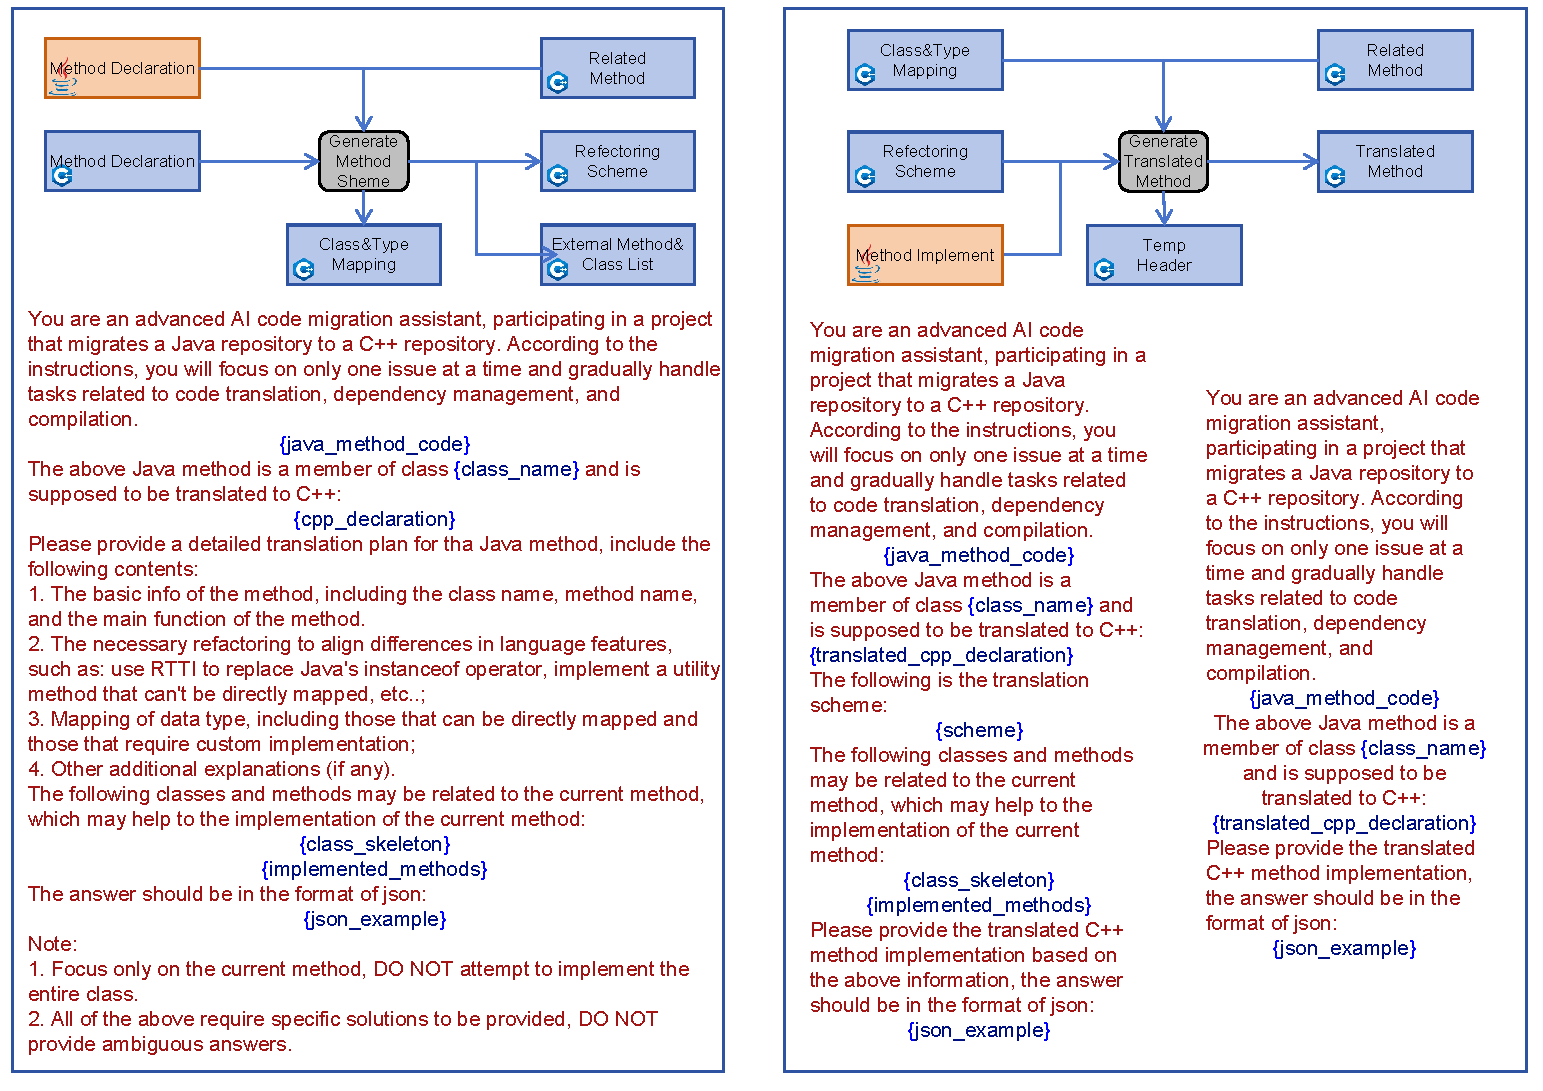
\includegraphics[width=\textwidth]{figures/approach/method_translation_prompt.pdf}
  \caption{Method-level translation scheme and data flow. The bottom-up translation order ensures that callee methods are translated before callers, enabling context propagation where already-translated code serves as reference.}
  \label{fig:method-translation}
\end{figure*}

\subsection{Validation and Repair}

The final phase addresses compilation errors through an autonomous agent that iteratively analyzes, diagnoses, and fixes translation defects. This phase bridges the gap between syntactically correct translation and semantically correct, compilable code.

\subsubsection{Compilation Agent Architecture}

The Compilation Agent operates as a closed-loop system with four core capabilities accessed through a tool-use interface:
\begin{enumerate}
\item \textbf{compile}: Invoke the C++ compiler on a specific source file and capture the output
\item \textbf{read\_file}: Read the current contents of any source or header file
\item \textbf{write\_file}: Replace the contents of a file with modified code
\item \textbf{create\_file}: Generate new header or source files as needed
\end{enumerate}

The agent maintains a conversation history with the LLM, providing compilation errors as feedback and requesting fixes. This interactive process continues until compilation succeeds or maximum attempts are reached.

\subsubsection{Iterative Repair Process}

For each C++ source file in dependency order, the agent executes the following loop:
\begin{enumerate}
\item Invoke \texttt{compile} on the target source file
\item If compilation succeeds, proceed to the next file
\item Otherwise, provide the compilation error output to the LLM
\item The LLM analyzes the error and generates a response containing:
\begin{itemize}
\item A diagnosis of the root cause
\item A sequence of tool calls to fix the issue (e.g., \texttt{read\_file} to examine code, \texttt{write\_file} to apply corrections, \texttt{create\_file} to add missing headers)
\item A status indicator for whether further iterations are needed
\end{itemize}
\item Execute the requested tool calls
\item Repeat from step 1
\end{enumerate}

This approach enables automatic resolution of common translation errors including:
\begin{itemize}
\item Missing header includes
\item Type mismatches and implicit conversion issues
\item Template instantiation errors
\item Linker errors due to missing definitions
\end{itemize}

\begin{figure}[h]
\centering
\begin{tikzpicture}[
    node distance=0.7cm,
    box/.style={
        rectangle,
        draw=black,
        thick,
        fill=white,
        text width=2.2cm,
        align=center,
        minimum height=0.65cm,
        font=\footnotesize
    },
    decision/.style={
        diamond,
        draw=black,
        thick,
        fill=white,
        text width=1.5cm,
        align=center,
        aspect=2,
        font=\footnotesize
    },
    terminal/.style={
        rectangle,
        rounded corners=2mm,
        draw=black,
        thick,
        fill=gray!15,
        text width=1.5cm,
        align=center,
        minimum height=0.55cm,
        font=\footnotesize
    },
    llmbox/.style={
        rectangle,
        draw=black,
        thick,
        fill=yellow!12,
        text width=2.2cm,
        align=center,
        minimum height=0.65cm,
        font=\footnotesize
    },
    toolbox/.style={
        rectangle,
        draw=black,
        thick,
        fill=blue!10,
        text width=1.8cm,
        align=center,
        minimum height=0.55cm,
        font=\footnotesize
    },
    arrow/.style={
        ->,
        >=stealth,
        thick
    }
]

% Vertical single-column layout
\node[terminal] (start) {Start};
\node[box, below=of start] (compile) {Compile file};
\node[decision, below=of compile] (success) {Success?};
\node[terminal, below left=0.5cm and 1cm of success] (done) {Done};

\node[llmbox, below=0.5cm of success] (analyze) {LLM analyzes\\and fixes};
\node[toolbox, below=of analyze] (tools) {Execute tools};

\node[decision, right=1.2cm of tools] (maxAttempts) {Max\\attempts?};
\node[terminal, below=of maxAttempts] (failed) {Failed};

% Arrows
\draw[arrow] (start) -- (compile);
\draw[arrow] (compile) -- (success);
\draw[arrow] (success) -- node[above, font=\tiny] {yes} (done);
\draw[arrow] (success) -- node[left, font=\tiny] {no} (analyze);
\draw[arrow] (analyze) -- (tools);

\draw[arrow] (tools.east) -- (maxAttempts.west);
\draw[arrow] (maxAttempts) -- node[right, font=\tiny] {no} (compile.east);
\draw[arrow] (maxAttempts) -- node[right, font=\tiny] {yes} (failed);

\end{tikzpicture}
\caption{The compilation agent's iterative repair process.}
\label{fig:agent-repair}
\end{figure}

\subsection{Key Design Features}

\subsubsection{Bottom-Up Translation with Context Propagation}

The bottom-up translation order is the cornerstone of our approach, enabling context propagation that significantly improves translation quality. By translating callees before callers, we ensure that:

\begin{enumerate}
\item \textbf{Consistent API usage}: When translating a caller method, the LLM sees the exact signatures and usage patterns of already-translated callees, eliminating mismatches in function calls, parameter passing, and return value handling.

\item \textbf{Pattern reinforcement}: Common translation patterns (e.g., how \texttt{Optional<T>} is converted, how exceptions are handled) are established early in leaf methods and consistently propagated through the call graph, reducing ad-hoc decisions.

\item \textbf{Incremental complexity}: Simple methods (often with few dependencies) are translated first, establishing project-wide conventions before tackling complex methods with deep call stacks.
\end{enumerate}

This ordering is derived automatically from the call graph using topological sort (Kahn's algorithm), which groups methods into dependency layers where all methods in layer $i$ depend only on methods in layers $1$ through $i-1$.

\subsubsection{Dual-Pass Translation with Scheme Generation}

Each translation unit (Header and Method) undergoes two passes:
\begin{enumerate}
\item \textbf{Scheme Pass}: High-level planning without generating code. The LLM produces a structured document analyzing the translation requirements and specifying the strategy.
\item \textbf{Code Pass}: Implementation guided by the scheme. The LLM generates actual C++ code following the strategy established in the scheme.
\end{enumerate}

The two-pass approach provides several critical benefits:

\begin{itemize}
\item \textbf{Separation of concerns}: Strategic decisions (type mappings, refactoring needs, error handling approach) are made separately from tactical implementation, reducing cognitive load on the LLM.

\item \textbf{Explicit reasoning}: The scheme serves as an explanation of the translation approach, making the process more interpretable and enabling verification of design decisions before code generation.

\item \textbf{Error localization}: When translation errors occur, the scheme provides context for understanding the LLM's intent, facilitating more effective error diagnosis and correction.

\item \textbf{Template for consistency}: The scheme establishes conventions that can be referenced when translating related code (e.g., all methods in a class use the same type mappings specified in the Header scheme).
\end{itemize}

\subsubsection{Hierarchical Graph Representation}

The bipartite graph model (Headers and Methods) provides a clean separation between structural and behavioral aspects of the codebase:

\begin{itemize}
\item \textbf{Structural isolation}: Header translation focuses exclusively on type definitions, field declarations, and API contracts, without the complexity of method implementations.

\item \textbf{Behavioral independence}: Method translation operates on implementation logic separately from type definitions, with the translated Header providing a stable API contract.

\item \textbf{Explicit dependencies}: The graph captures both structural relationships (inheritance, type usage through imports) and behavioral relationships (method calls), enabling systematic translation ordering.
\end{itemize}

This representation maps naturally to the C++ compilation model (header files and implementation files), while accommodating Java's compilation unit structure (where multiple classes may reside in one source file).

\subsubsection{Heterogeneous Translation with Structural Adaptation}

Unlike traditional code translation approaches that aim for syntactic one-to-one mapping, the translated codebase may exhibit structural differences from the source while preserving functional equivalence. This design philosophy is enabled by two key features:

\begin{itemize}
\item \textbf{Scheme-driven refactoring}: During scheme generation, the LLM can propose structural transformations that better align with target language idioms. These refactoring decisions are made before code generation, allowing systematic reorganization of the codebase structure.

\item \textbf{Header-level flexibility}: The Header translation phase operates at the type-system level, where the LLM has broad freedom to redesign APIs, reorganize inheritance hierarchies, or adopt entirely different architectural patterns (e.g., replacing inheritance with templates, converting classes to namespaces).
\end{itemize}

This approach is particularly advantageous for cross-paradigm translation (e.g., Java to C++), where mechanical preservation of source structure often results in non-idiomatic code. For example:
\begin{itemize}
\item Java's single-inheritance class hierarchy may be restructured using C++ multiple inheritance or CRTP (Curiously Recurring Template Pattern)
\item Runtime polymorphism based on interfaces may be partially replaced with compile-time polymorphism using templates
\item Reflection-based designs may be restructured to use compile-time type traits and constexpr metaprogramming
\item Exception-heavy error handling may be converted to RAII-based resource management with optional return values
\end{itemize}

By granting the LLM freedom to adapt project structure to target language conventions, heterogeneous translation produces more maintainable and idiomatic code than rigid structure-preserving approaches.
